\documentclass{article}
\usepackage{graphicx} % Required for inserting images

\title{CMM HW4}
\author{Xuanhao Lin}
\date{November 14 2023}

\begin{document}

\maketitle

\section{Random Numbers}
\subsection{Part 1}
\paragraph{
The probability distributions of evenly distributed random numbers are shown as Figure 1 and Figure 2. We can clearly find that the random numbers distribute more evenly with larger sampling number.
}
\begin{figure}[htbp]
    \centering
    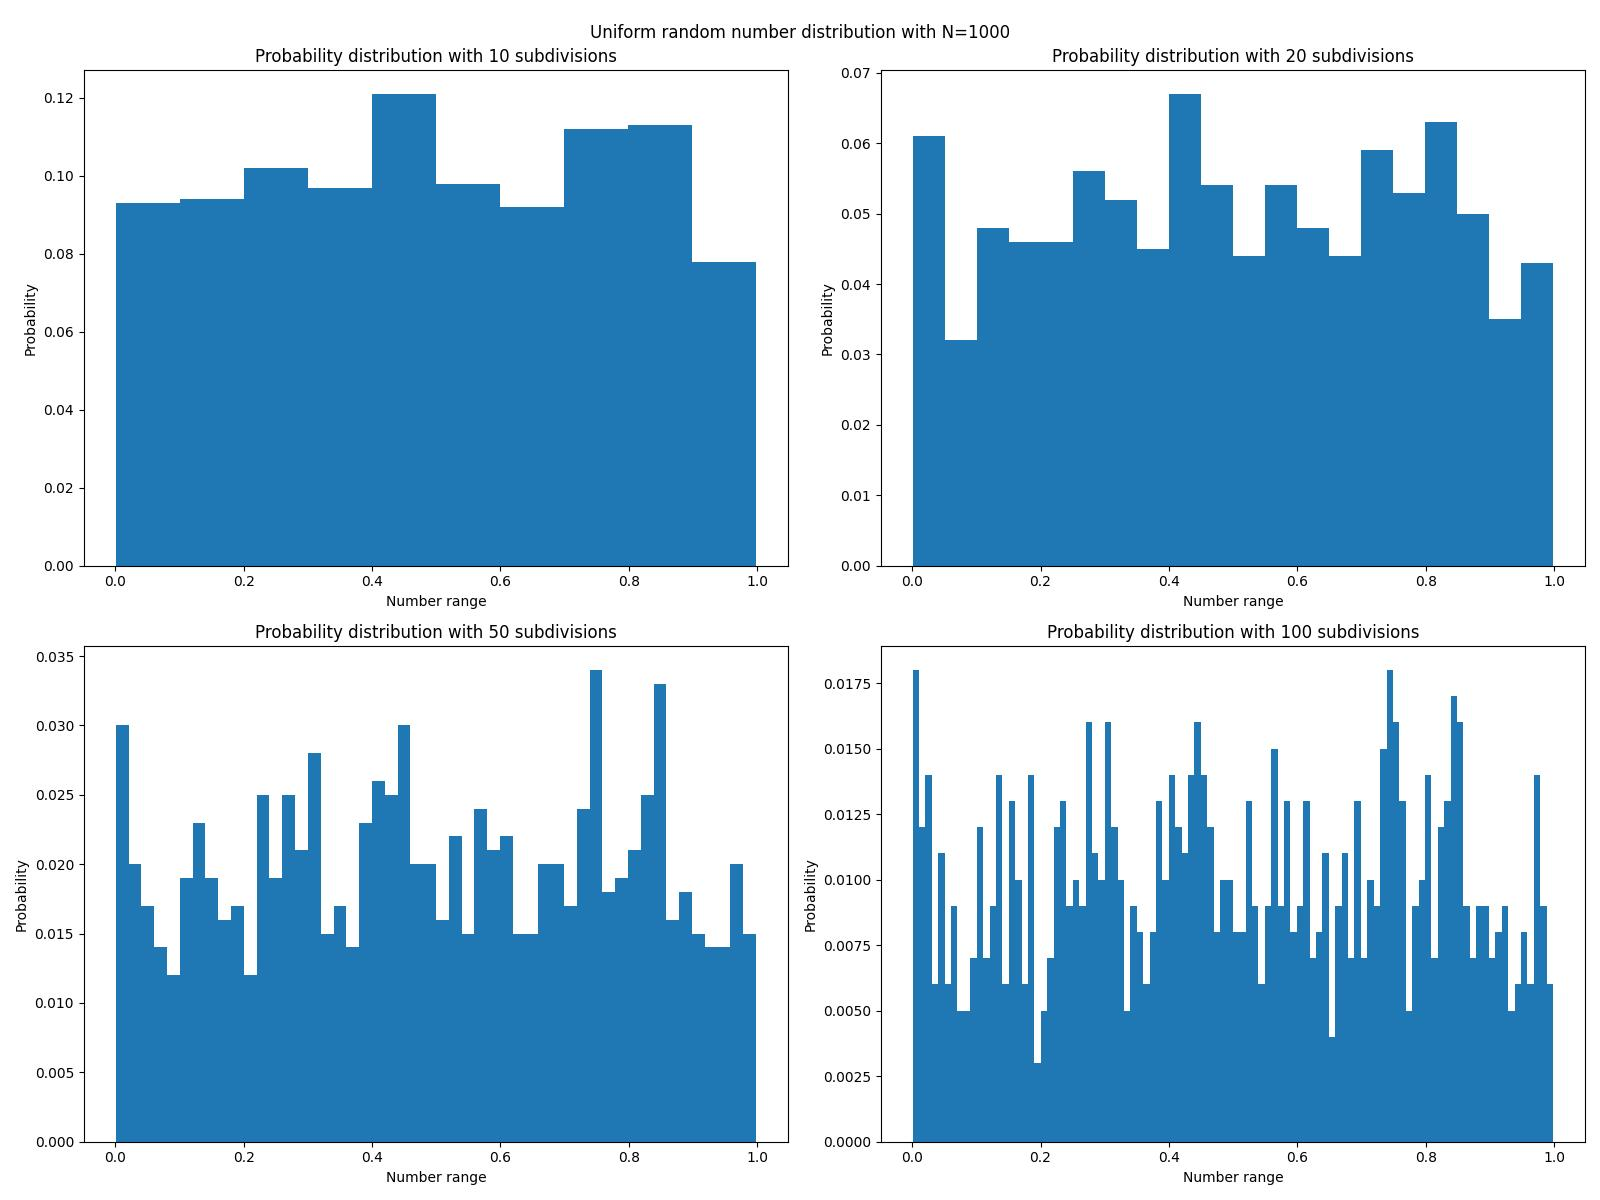
\includegraphics[width=0.5\linewidth]{Part1_1_N=1000.jpeg}
    \caption{Uniform random distribution with N=1000}
\end{figure}
\begin{figure}[htbp]
    \centering
    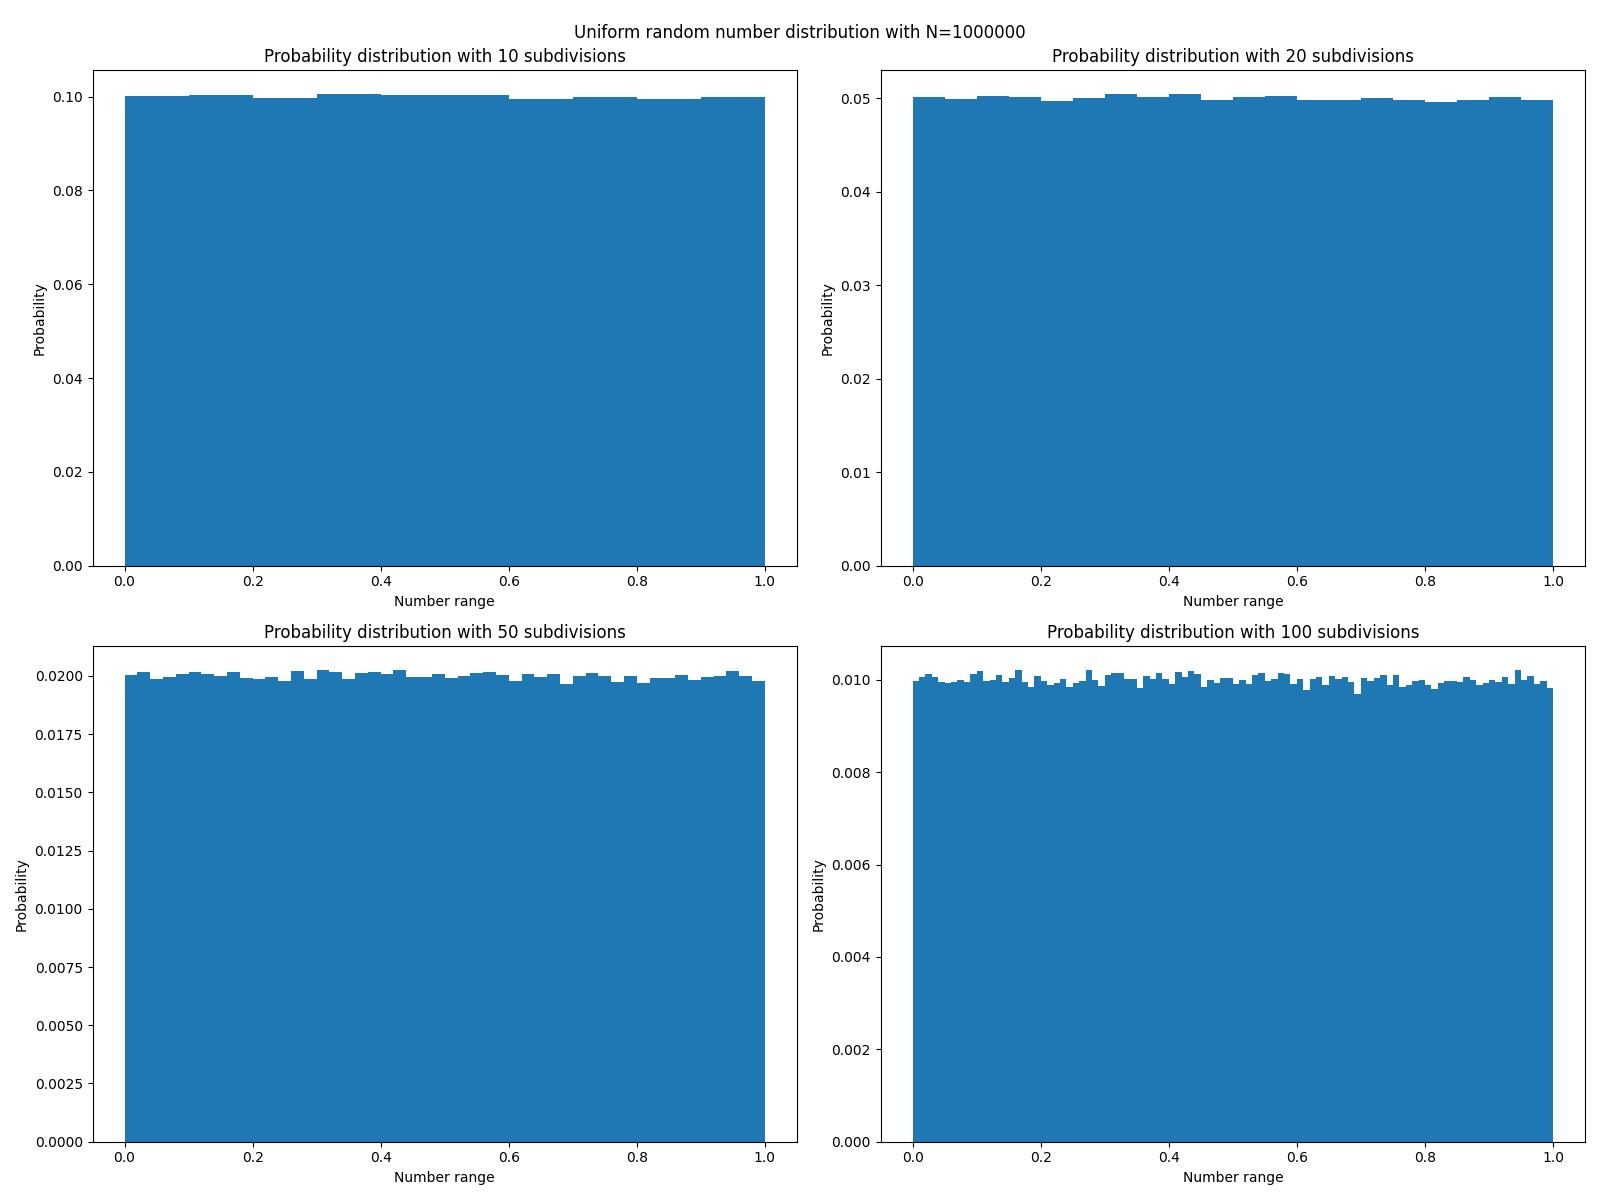
\includegraphics[width=0.5\linewidth]{Part1_1_N=1000000.jpeg}
    \caption{Uniform random distribution with N=1000000}
\end{figure}[htbp]
\subsection{Part 2}
\paragraph{
To generate non-uniform distributed random numbers, I used the rejection method mentioned in class. By comparing Figure 3 and Figure 4, it is obvious that the random numbers can satisfy the required distribution with large enough samplings.
}
\begin{figure}[htbp]
    \centering
    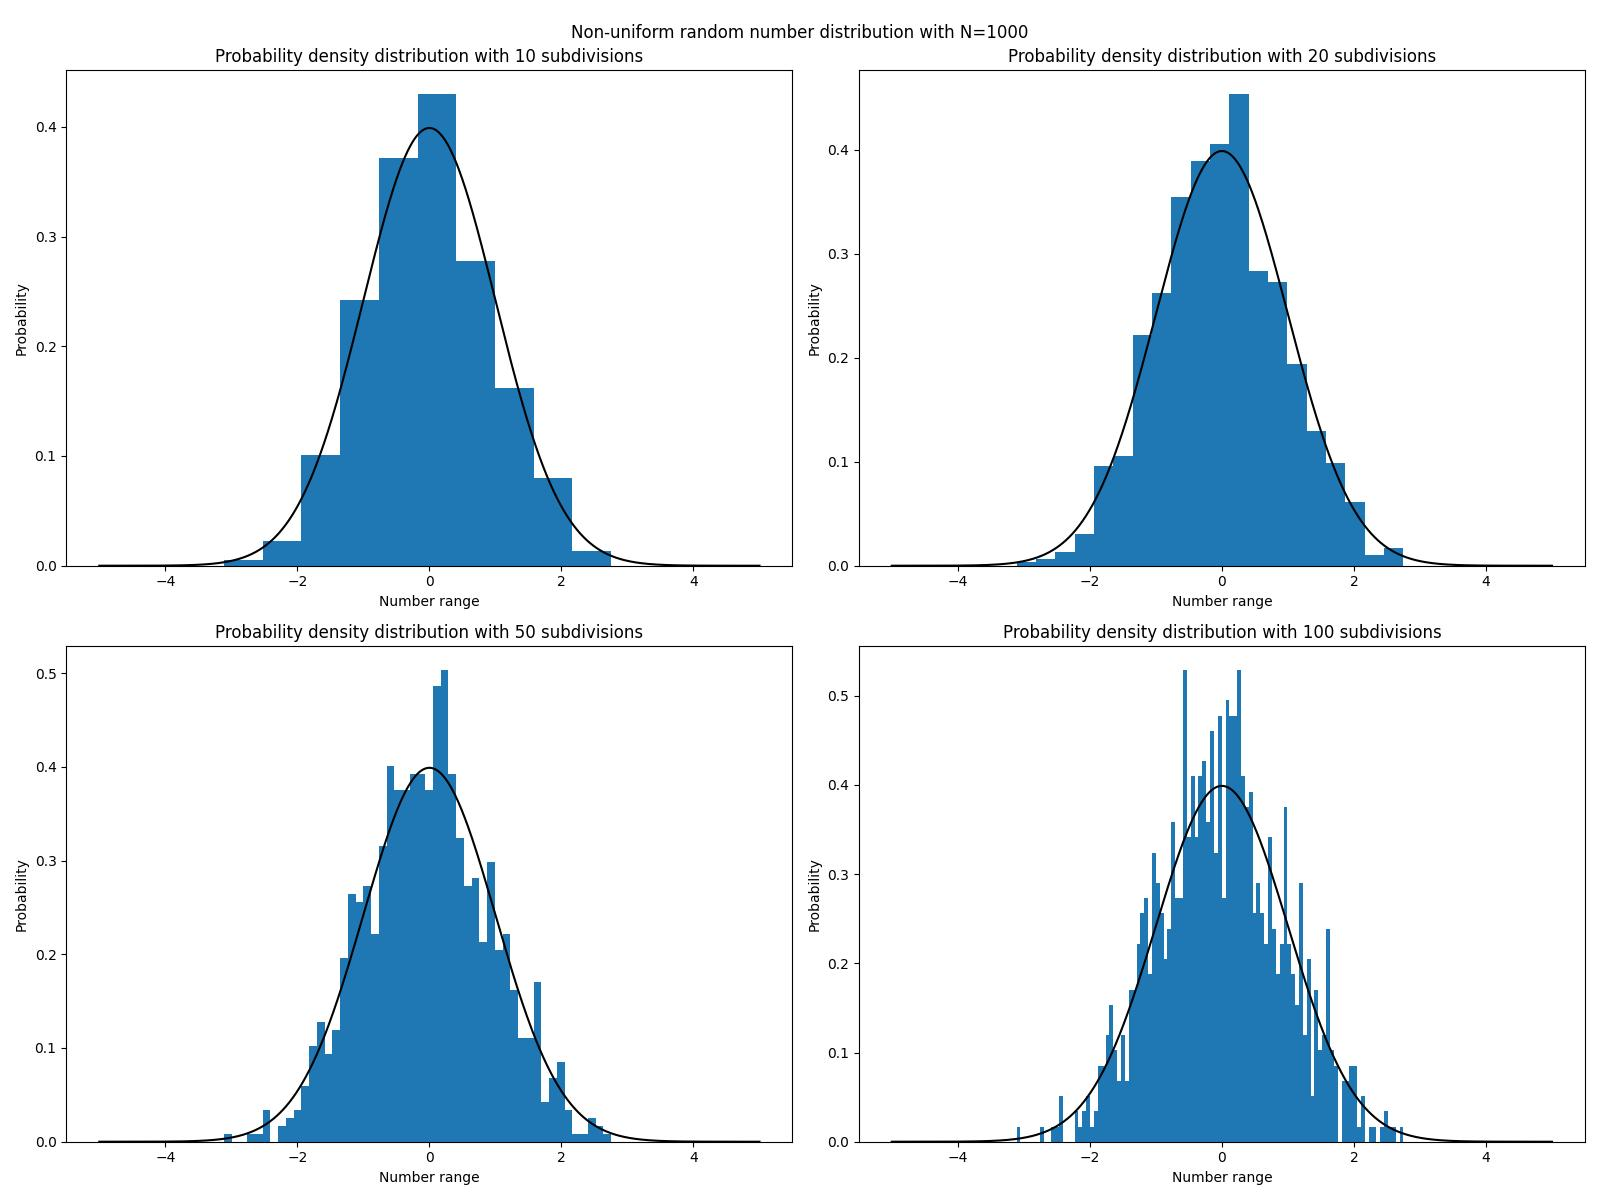
\includegraphics[width=0.5\linewidth]{Part1_2_N=1000.jpeg}
    \caption{Non-uniform random distribution with N=1000}
\end{figure}
\begin{figure}[htbp]
    \centering
    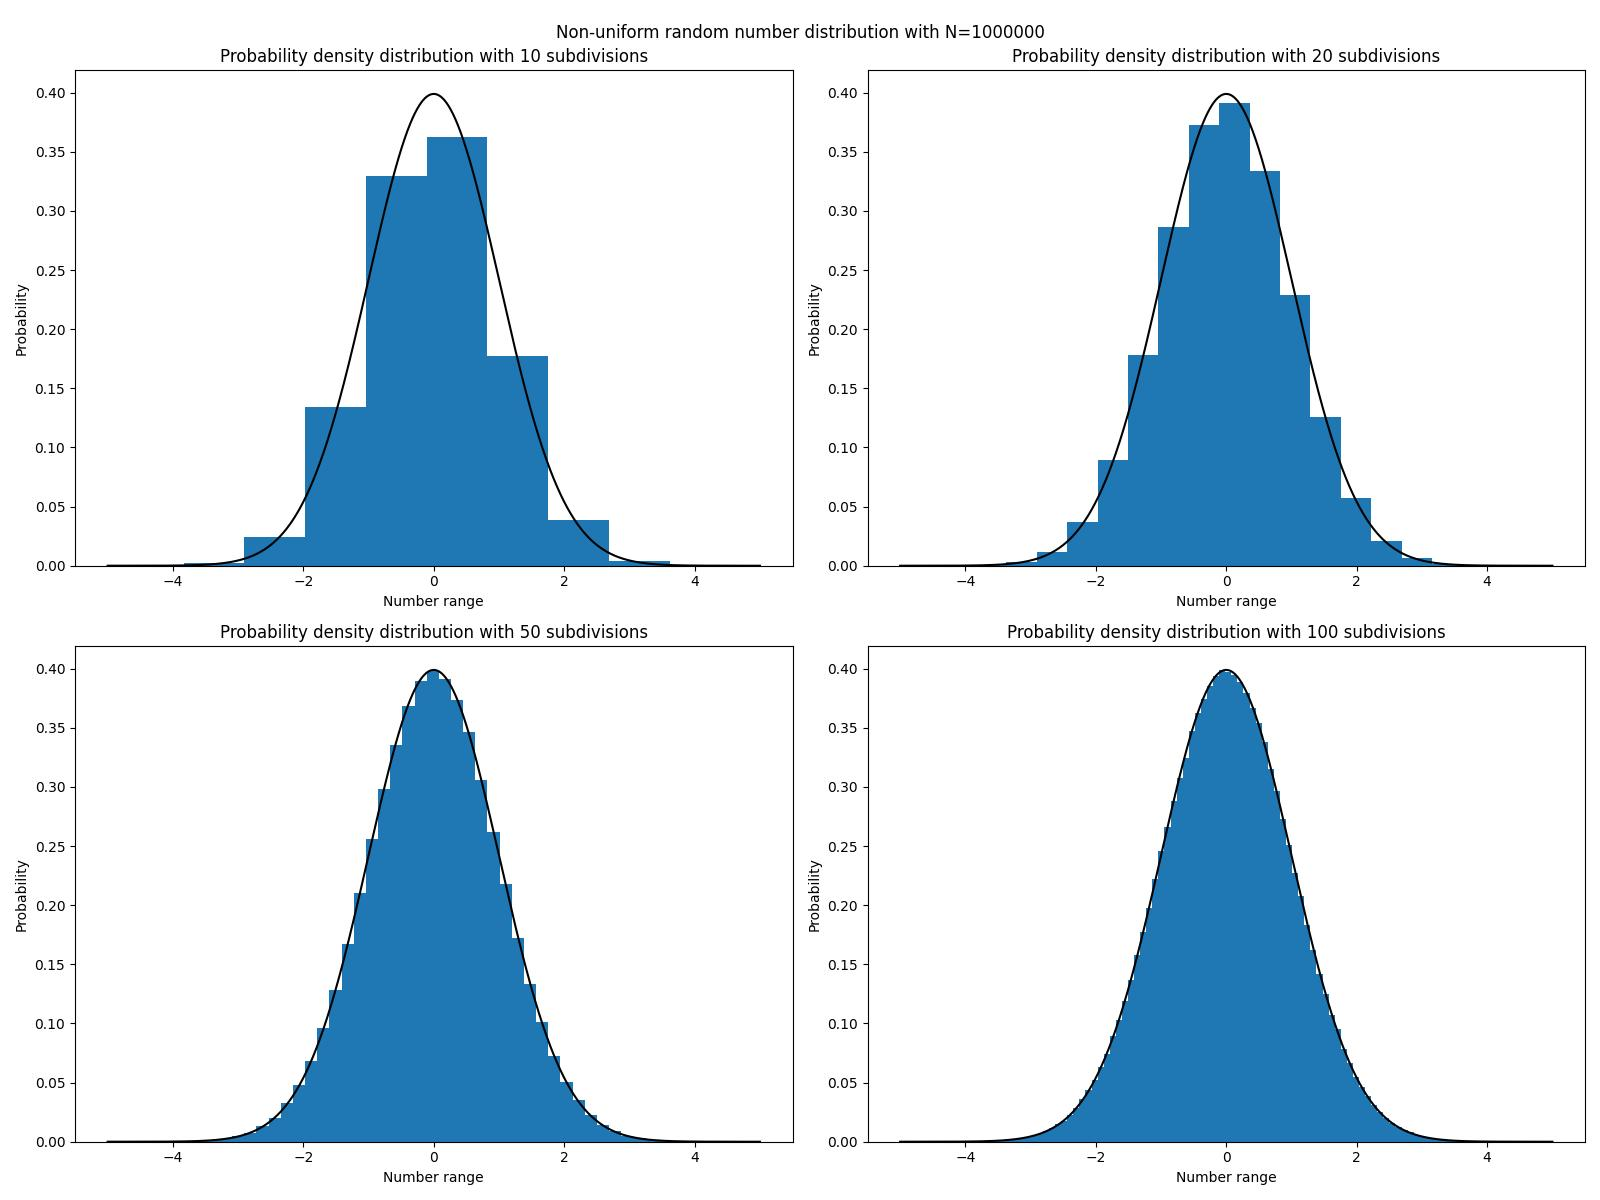
\includegraphics[width=0.5\linewidth]{Part1_2_N=1000000.jpeg}
    \caption{Non-uniform random distribution with N=1000000}
\end{figure}
\section{2D Random Walk}
\subsection{Part 1}
\paragraph{
The results are shown as Figure 5-9.
}
\begin{figure}[htbp]
    \centering
    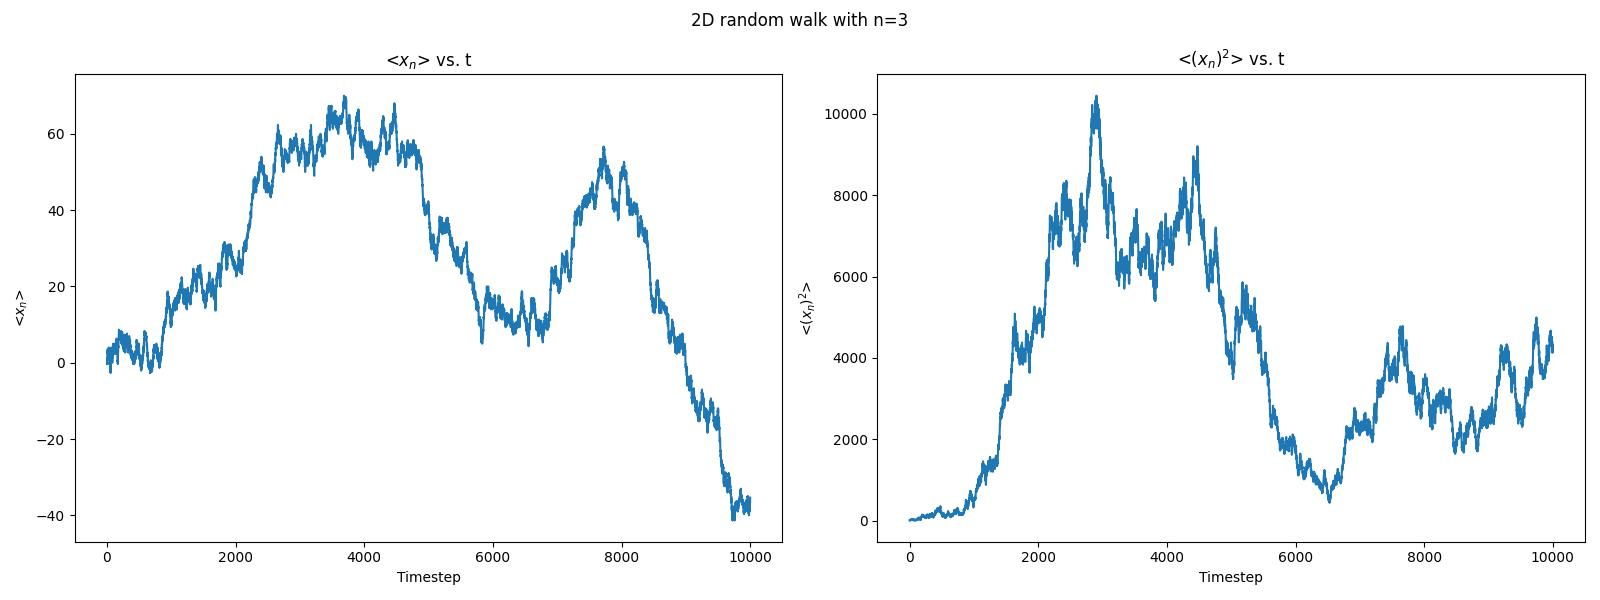
\includegraphics[width=0.5\linewidth]{Part2_1_n=3.jpeg}
    \caption{2D random walk with n=3}
\end{figure}
\begin{figure}[htbp]
    \centering
    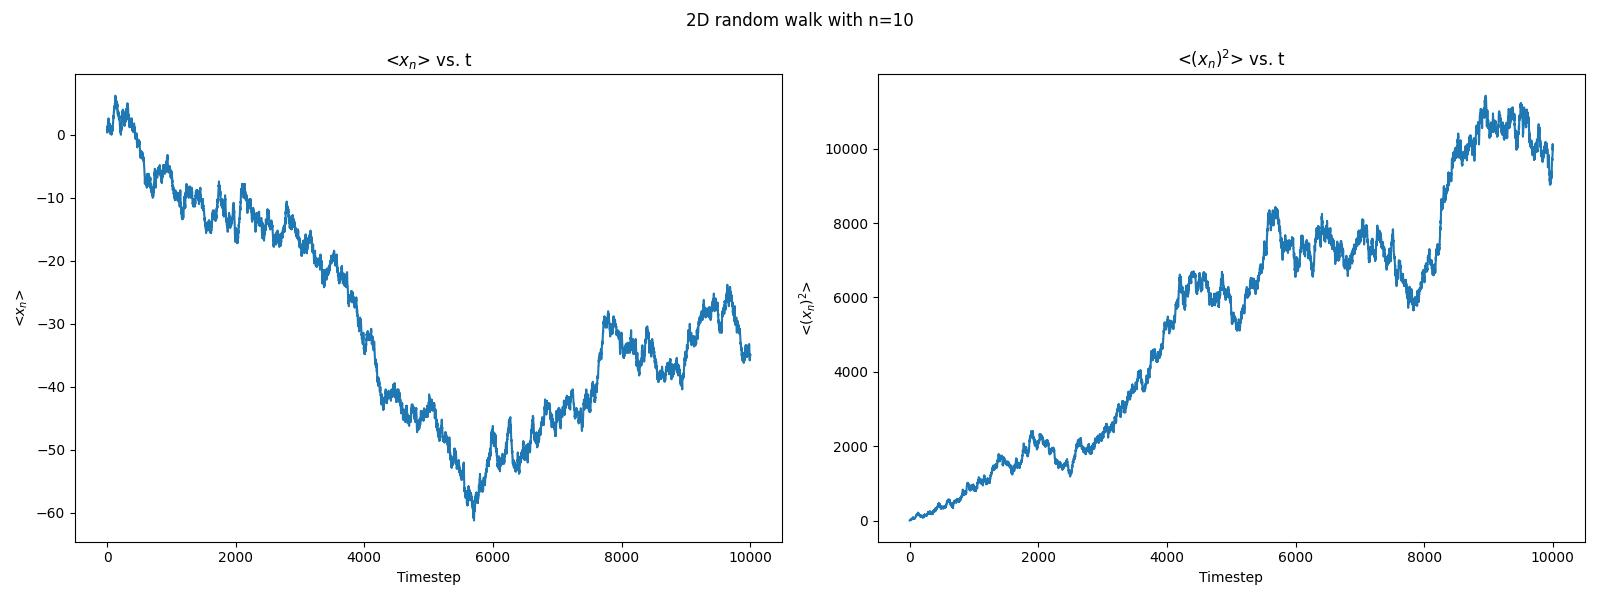
\includegraphics[width=0.5\linewidth]{Part2_1_n=10.jpeg}
    \caption{2D random walk with n=10}
\end{figure}
\begin{figure}[htbp]
    \centering
    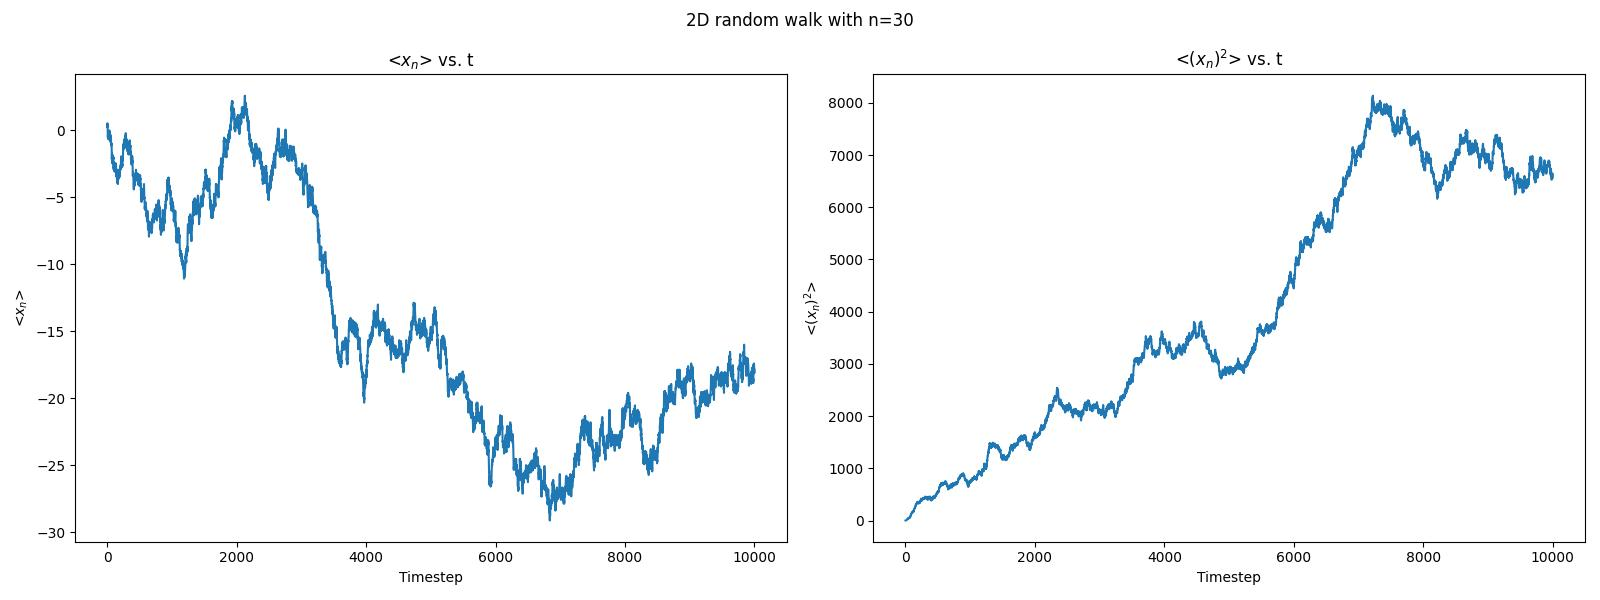
\includegraphics[width=0.5\linewidth]{Part2_1_n=30.jpeg}
    \caption{2D random walk with n=30}
\end{figure}
\begin{figure}[htbp]
    \centering
    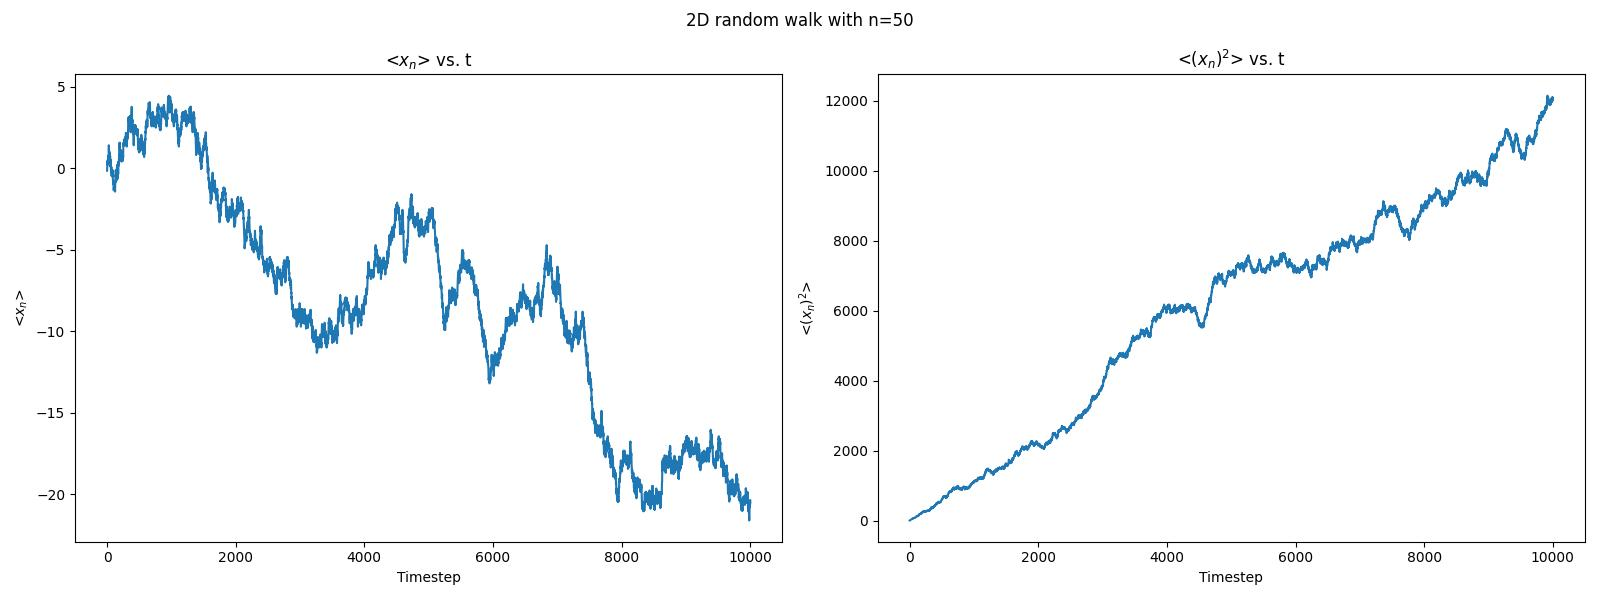
\includegraphics[width=0.5\linewidth]{Part2_1_n=50.jpeg}
    \caption{2D random walk with n=50}
\end{figure}
\begin{figure}[htbp]
    \centering
    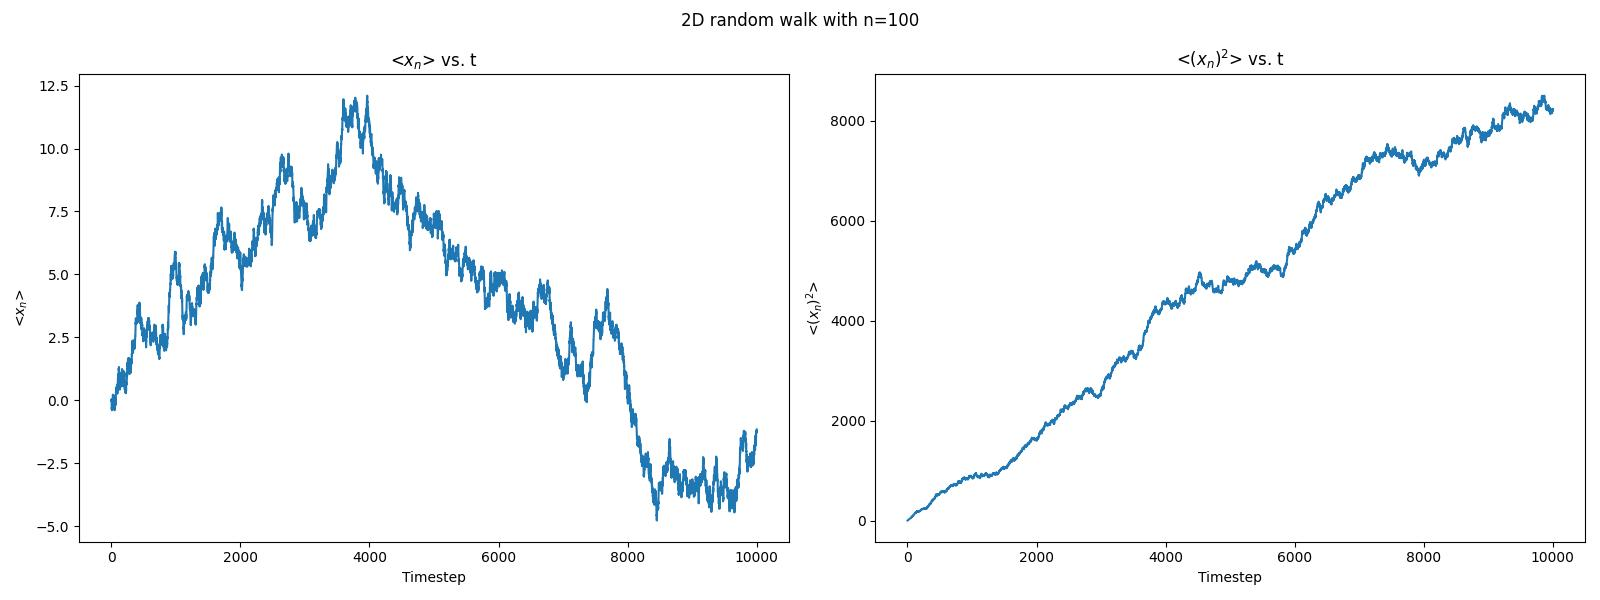
\includegraphics[width=0.5\linewidth]{Part2_1_n=100.jpeg}
    \caption{2D random walk with n=100}
\end{figure}
\subsection{Part 2}
\paragraph{
From Figure 10, we can find that the motion is diffusive since $<r^2>$ is roughly proportional to t. And the diffusion constant can be easily determined as $\frac{1}{2}$ from \(<r^2>=2Dt\).
}
\begin{figure}[htbp]
    \centering
    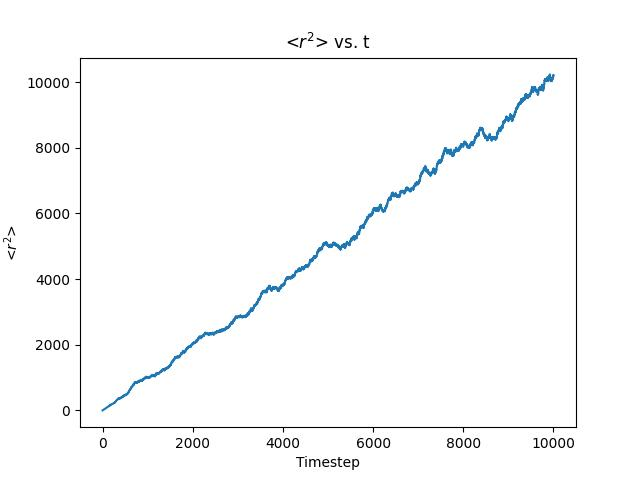
\includegraphics[width=0.5\linewidth]{Part2_2.jpeg}
    \caption{$<r^2>$ vs. t}
\end{figure}
\section{Diffusion Equation}
\subsection{Part 1}
\paragraph{
The expectation value \(<x^2>=\int_{\infty}^{\infty}x^2p(x,t)dx\). By replacement of variable: \(k=\frac{x^2}{2\sigma^2}\), we can obtain:
\[<x^2>=\frac{\sigma(t)^2}{\sqrt{\pi}}\int_{\infty}^{\infty}e^{-k^2}dk\]
The latter part is known as the Gaussian integral which is equal to $\sqrt{\pi}$. Therefore, we finally get:
\[<x^2>=\sigma(t)^2\]
}
\subsection{Part 2}
\paragraph{
After numerically calculating the !D diffusion equation, we can plot the results as Figure 11. We can observe that the values obtained from curve fitting have very good agreements to the theoretical values.
}
\begin{figure}[htbp]
    \centering
    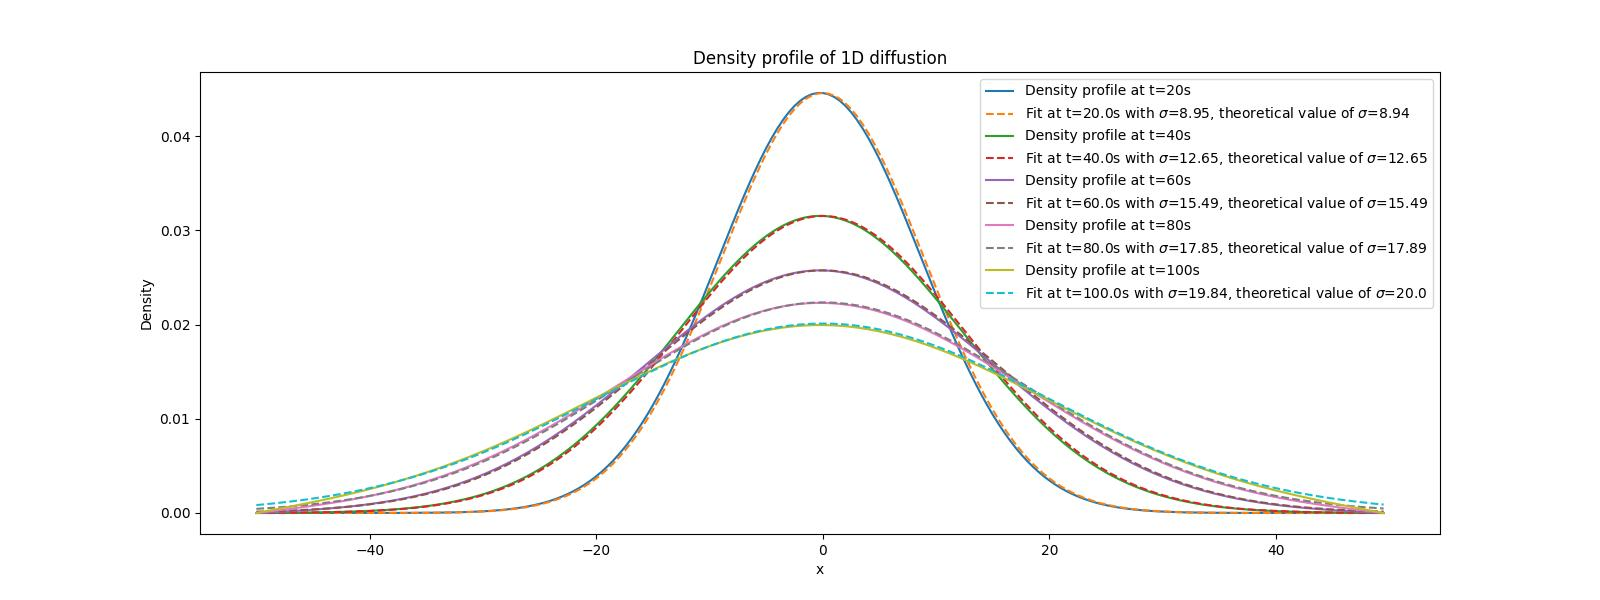
\includegraphics[width=0.5\linewidth]{Part3_2.jpeg}
    \caption{Density profile of !D diffusion}
\end{figure}
\section{Mixing of Two Gases}
\subsection{Part 1}
\paragraph{
This is a part giving instructions how to build up the model.
}
\subsection{Part 2}
\paragraph{
After iterating enough time step, we can obtain Figure 12. Also, Figure 13-17 show some configurations during the process, which clearly shows the distribution of the gas particles.
}
\begin{figure}[htbp]
    \centering
    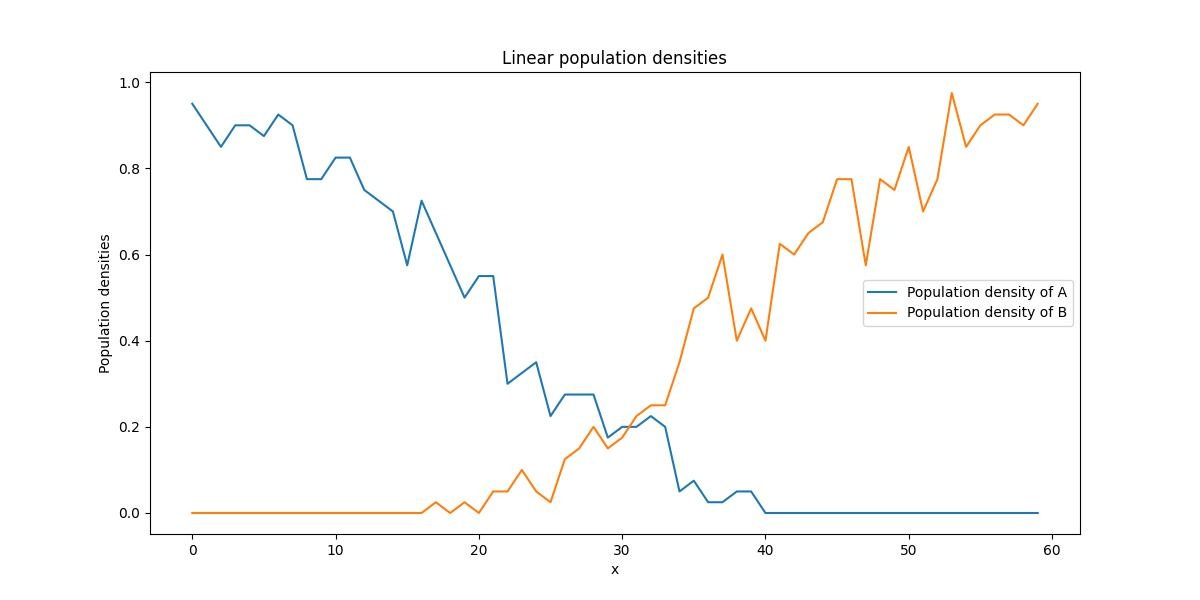
\includegraphics[width=0.5\linewidth]{Part4_1.jpeg}
    \caption{Linear population densities}
\end{figure}
\begin{figure}[htbp]
    \centering
    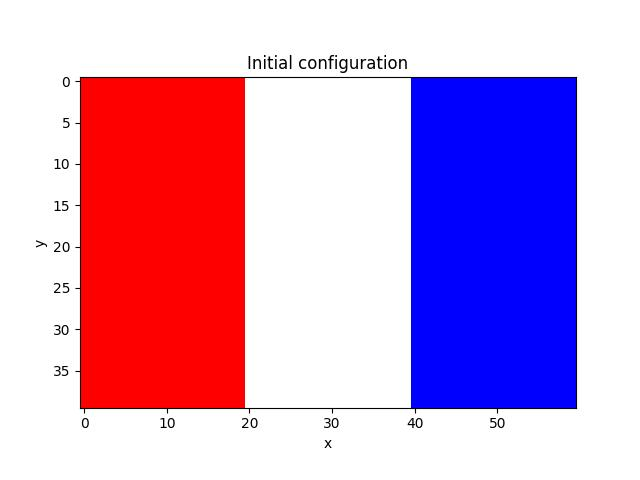
\includegraphics[width=0.5\linewidth]{Part_4_2_timestep=0.jpeg}
    \caption{Initial configuration}
\end{figure}
\begin{figure}[htbp]
    \centering
    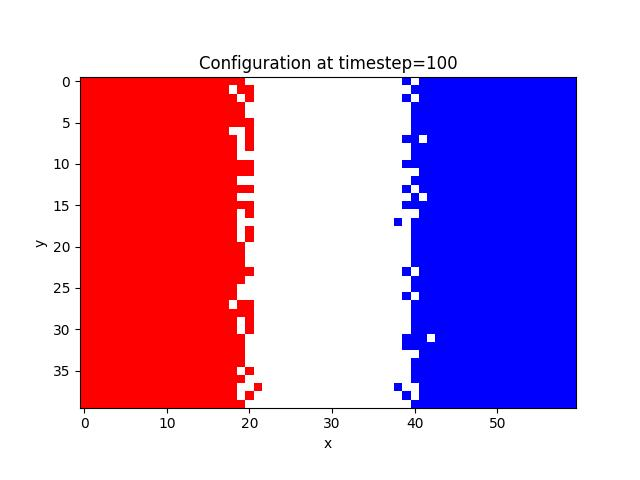
\includegraphics[width=0.5\linewidth]{Part_4_2_timestep=100.jpeg}
    \caption{Configuration at timestep=100}
\end{figure}
\begin{figure}[htbp]
    \centering
    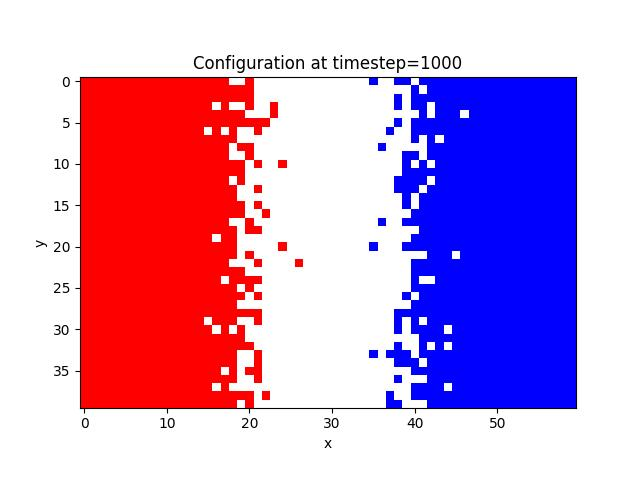
\includegraphics[width=0.5\linewidth]{Part_4_2_timestep=1000.jpeg}
    \caption{Configuration at timestep=1000}
\end{figure}
\begin{figure}[htbp]
    \centering
    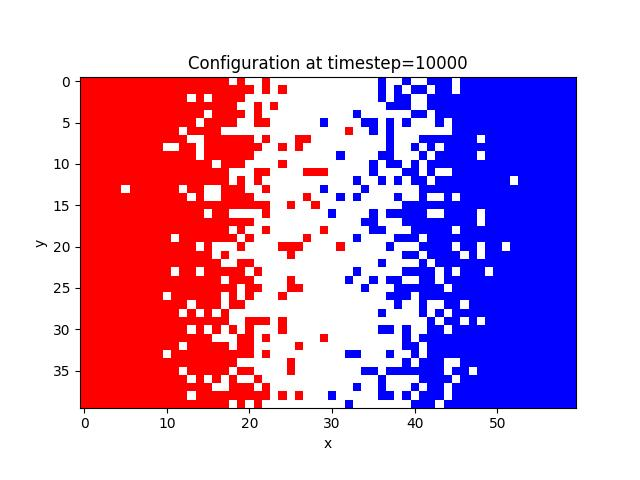
\includegraphics[width=0.5\linewidth]{Part_4_2_timestep=10000.jpeg}
    \caption{Configuration at timestep=10000}
\end{figure}
\begin{figure}[htbp]
    \centering
    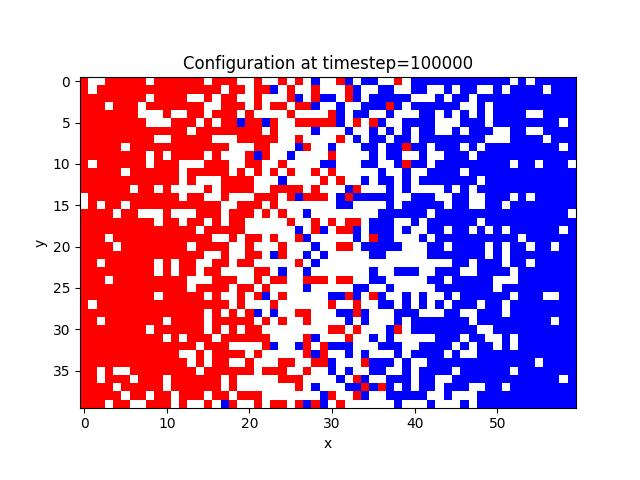
\includegraphics[width=0.5\linewidth]{Part_4_2_timestep=100000.jpeg}
    \caption{Configuration at timestep=100000}
\end{figure}
\subsection{Part 3}
\paragraph{
By averaging the densities over 100 trials, we can get the result shown as Figure 18. The curves become smooth, and they show a great agreement to the theoretical curve which corresponds to the mixing of two gases.
}
\begin{figure}[htbp]
    \centering
    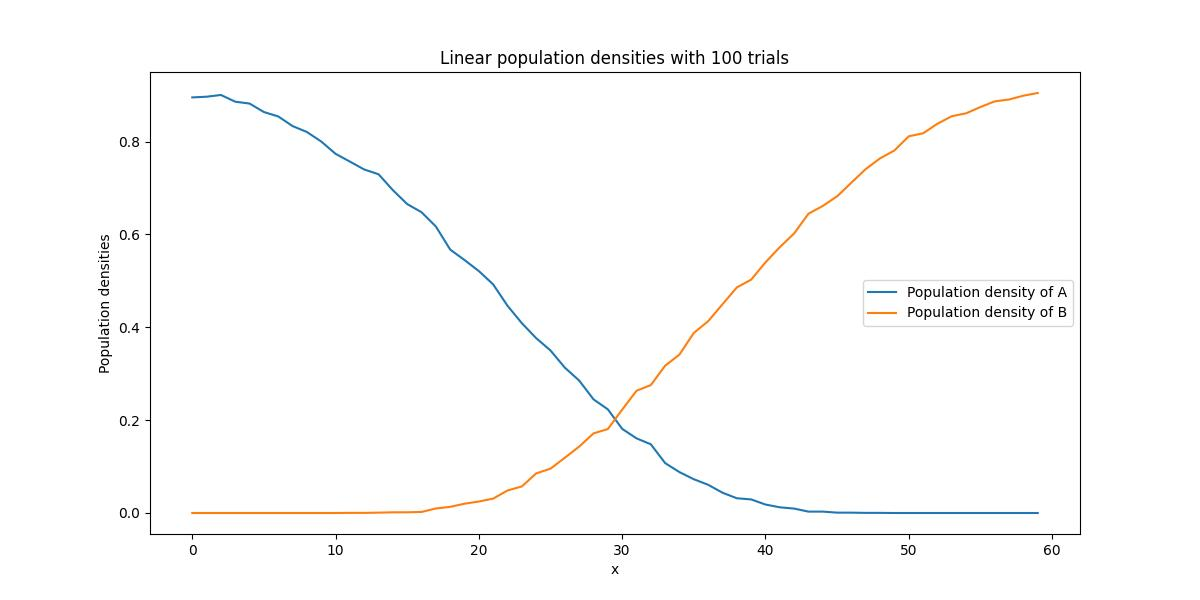
\includegraphics[width=0.5\linewidth]{Part4_3.jpeg}
    \caption{Linear population densities with 100 trials}
\end{figure}
\end{document}
